\documentclass[11pt]{article}
\usepackage[margin=0.85in]{geometry}
\usepackage[T1]{fontenc}
\usepackage[utf8]{inputenc}
\usepackage{amsmath,amssymb,booktabs,longtable,graphicx}
\usepackage[round]{natbib}
\usepackage[hidelinks]{hyperref}
\usepackage{microtype}
\setlength{\emergencystretch}{3em}
\title{RC-QASyn: Auditable Evidence, Coverage-Aware Construction and Bounded Repair for Synthetic Tabular Data}
\author{[Author names pending]\\[0.3em]\small [Department, institution and contact pending]}
\date{Research manuscript draft --- 19 October 2026}
\begin{document}
\maketitle
\begin{abstract}
Synthetic tabular records can be parseable while failing a source schema, statistically unusual without being invalid, or individually plausible while providing redundant dataset coverage. RC-QASyn separates these questions in an auditable prototype. It binds generated occurrences to sources, distinguishes authoritative structure from local/global TRAIN support, reports descriptive dependent evidence, constructs fixed-budget provisional datasets and applies narrowly approved integer-only repair. A three-dataset historical study contains 601 occurrences and 75 structural rejects. Only 54 qualify for repair; all become structurally compatible, with 49 provisional passes and five review-required outcomes under the unchanged shadow policy. Twenty-one rejects remain ineligible. Construction and 138 predeclared task-utility comparisons are reproducible; 114 return results and 24 are explicitly unavailable. Coverage and classifier utility do not improve uniformly. The 120-record validity cohort has no human-final approvals, so validity calibration and human-ground-truth performance remain unavailable. The contribution is an inspectable workflow and bounded exploratory evidence, not proof of semantic validity, calibrated risk or generalization.
\end{abstract}
\noindent\textbf{Keywords:} synthetic tabular data; imbalanced classification; provenance; evidence fusion; coverage; bounded repair; reproducibility.

\section{Introduction}
Synthetic tabular generation is attractive when minority examples are scarce, but useful data require more than fluent output or parser success. A candidate may omit its target, violate an integer declaration, repeat another example, or concentrate in a dense TRAIN region. Conversely, rarity and distance from observed values do not establish invalidity. These distinctions matter when synthetic records train classifiers.

RC-QASyn preserves authoritative constraints, statistical support, uncertainty, dataset contribution and task utility as different quantities. An audit trail connects results to original occurrences and versioned configurations. Small deterministic components are preferred over learned fusion whose approved supervision is unavailable.

This draft covers six implemented phases. Evaluation stabilization and source reconciliation precede heterogeneous evidence; descriptive fusion and shadow admission precede construction; bounded repair creates derived candidates without altering history. Negative and unavailable outcomes are retained. Scientific acceptance remains pending: validity review, original target meanings and official calibration are unresolved. The project acronym is retained without claiming operationally calibrated validity.

\section{Problem formulation and research objectives}
Let $T$ be frozen real TRAIN, $E$ historical real TEST, and $G=\{(o_i,x_i,y_i)\}$ the generated stream. Each $o_i$ identifies a physical source occurrence; equal payloads at different positions remain distinct. Missing $y_i$ remains missing, never replaced by conditioning. A ledger binds each occurrence to source/payload fingerprints.

We ask which defects are authoritative, how local/global support relate, how fixed-budget selection changes coverage/redundancy, and what bounded repair changes structurally, geometrically and in utility. Unapproved agent labels do not answer these questions. The output is a reproducible exploratory dataset, not a claim that every selected record is truly valid.

\section{Related work}
CTGAN addresses conditional mixed tabular generation \citep{xu2019ctgan}; TabDDPM studies diffusion-based tabular modeling \citep{kotelnikov2023tabddpm}; GReaT studies language-model generation \citep{borisov2023great}. These motivate the setting. We do not implement or compare those generators, and this historical stream establishes no superiority over them.

Synthetic-data evaluation can separate fidelity, diversity and generalization \citep{alaa2022faithful}. Our coverage and duplication measures are narrower diagnostics, not implementations of that work's metrics or privacy guarantees. Constraint-aware generation illustrates that distributional resemblance need not imply logical compliance \citep{stoian2024realistic}; our prototype instead audits justified declarations after generation and permits narrowly bounded correction.

Calibration concerns confidence/outcome agreement \citep{guo2017calibration}. Candidate percentiles lack that interpretation without approved labels and eligible evaluation. We retain a gated future interface, refusing real-cohort fitting. Language-model judge studies identify judge limitations \citep{zheng2023judging}; conversational results do not establish tabular-critic error rates. Surveys connect generation, curation and evaluation \citep{long2024survey}. We make these stages traceable in this prototype, without comprehensive novelty or state-of-the-art claims.

\section{RC-QASyn methodology and architecture}
The implemented flow is source-bound generation $\rightarrow$ ground-truth specification $\rightarrow$ heterogeneous evidence $\rightarrow$ descriptive fusion and shadow admission $\rightarrow$ coverage-aware construction $\rightarrow$ bounded repair/reevaluation $\rightarrow$ task evaluation and reporting. Repair also feeds separately versioned construction; it never overwrites the original sequence.

\subsection{Generation contract, frozen controls and review ledger}
The provider request includes schema and class conditioning. The parser extracts objects; integration stores actual payloads. Conditioning and \texttt{requested\_class} do not substitute for missing payload class in a complete labeled record. Raw parser survival is weaker than complete-record validity. B1 is the frozen generation-only acceptance control, B2 the deterministic validator, and B3 the recorded provider-critic control. Later evidence does not rewrite these controls.

Reconciliation retains all 601 positions, the corrected 120-record cohort, 40-record review overlap and row-94 linkage to occurrence 1. Specifications separate source declarations from unresolved meaning. The research ledger is source-bound CSV/JSON with explicit human-review status, not cryptographic authentication against malicious same-permission actors. Proposals remain AGENT and pending. Technical consistency is not personal supervisor inspection or label approval.

\subsection{M2 authoritative and statistical evidence}
Structure checks mandatory features/class, primitives, nominal values, undeclared fields and source integer declarations. Substantiated authoritative defects can reject. Absence of demonstrated violations does not establish VALID. Unsupported evidence propagates uncertainty. Ranges, duplicates, rarity and model disagreement do not become physical constraints.

For $p$ features, use the frozen TRAIN mixed distance
\begin{equation}
d(x,t)=\frac1p\sum_{j=1}^p\delta_j(x_j,t_j),\quad
\delta_j=\begin{cases}\min(|x_j-t_j|/R_j,1),&j\text{ numeric},R_j>0,\\
\mathbf1[x_j\ne t_j],&j\text{ nominal or }R_j=0.\end{cases}
\end{equation}
$R_j$ is TRAIN span; class is excluded. Local support is $L_k(x)=k'^{-1}\sum_{t\in N_{k'}(x)}d(x,t)$, $k'=\min(k,|T_s|)$, with supported TRAIN reference $T_s$. Ties use original row identity. Baseline $k=5$; same-literal-class diagnostics are separate. Unsupported features cause unavailability.

Global evidence robust-scales numeric features by TRAIN median/IQR, falling back to span then one, and one-hot encodes TRAIN nominal categories. For encoded $z$, mean $\mu$, sample covariance $S$, shrinkage $\alpha$ and ridge $\lambda$,
\begin{equation}
\Sigma_{\alpha,\lambda}=(1-\alpha)S+\alpha\operatorname{diag}(S)+\lambda I,\quad
Q(x)=\sqrt{\max(0,(z-\mu)^\top\Sigma_{\alpha,\lambda}^{-1}(z-\mu))/D}.
\end{equation}
$D$ is encoded dimension. Baseline $\alpha=.10$; the baseline ridge is $10^{-8}$. Unseen categories can make global evidence unavailable. Elliptical consistency is not a physical law; TRAIN self-tail fractions are resubstitution diagnostics, not calibrated p-values. Five configurations vary $k$ or shrinkage without TEST selection.

\subsection{M4 descriptive normalization and dependence}
For dataset/family reference scores $A_f$ from original candidates,
\begin{equation}
u_f(s)=\frac{\#\{a\in A_f:a<s\}+\tfrac12\#\{a\in A_f:a=s\}}{|A_f|}.
\end{equation}
Larger means weaker support. This mid-distribution handles ties; references below minimum ten and missing scores remain explicit. The reference is historical candidate scores, not human validity or TEST. Original scores include themselves; derived queries never join it.

Report $U_{\max}=\max(u_L,u_Q)$ and $U_{\min}=\min(u_L,u_Q)$ only with both scores. These are uncalibrated indices. Rank correlation, concern union/intersection, disagreement and tail Jaccard are reported. We neither multiply probabilities nor assume independence or learn weights from agent labels. Actual calibration returns \texttt{NOT\_ELIGIBLE\_UNAPPROVED\_LABELS}. Synthetic eligible fixtures test the future interface, not real calibration.

\subsection{M5 conservative shadow decisions}
Precedence: authoritative defect $\Rightarrow$ REJECT\_STRUCTURAL; unavailable required evidence $\Rightarrow$ ABSTAIN; partial structure or any configured percentile at least $q$ $\Rightarrow$ REVIEW\_REQUIRED; otherwise PROVISIONAL\_PASS. Structure/local/global/combined policies are evaluated, with combined $q=.80,.95$ sensitivities around primary $.90$. Cutoffs are descriptive predeclared parameters. Outliers are never hard INVALID; provisional passes are never human VALID. Historical acceptance remains unchanged.

\subsection{M7 coverage-aware set construction}
Eligibility requires complete payloads and frozen provisional pass. Let $\mathcal R$ be distinct TRAIN (feature-payload, literal-class) regions, retaining first-source representatives so duplicates do not multiply the objective. At radius $r=.05$, $h_t(S)=\mathbf1[\min_{s\in S}d(s,t)\le r]$, $h_t(\varnothing)=0$. Define
\begin{equation}
C_{\mathcal R}(S)=\frac1{|\mathcal R|}\sum_{t\in\mathcal R}h_t(S),\qquad
C_{bal}(S)=\sum_{t\in\mathcal R}\frac{h_t(S)}{K n_{y_t}}.
\end{equation}
$K$ is represented class count and $n_y$ its region count. Also report TRAIN-row and distinct-feature coverage. Class-free geometry means any-class coverage differs from same-literal-class minority coverage.

Compare four selectors at budget $b$: earliest source order; farthest-first maximizing $\min_{z\in S}d(s,z)$; greedy uniform marginal coverage; and quality-constrained balanced coverage. The last prohibits repeated feature payloads and fills minority quota $\lfloor .5b\rfloor$ first, capped by distinct minority availability. Its lexicographic key is balanced marginal gain, fewer selected neighbors within $.01$, larger minimum separation, smaller frozen $U_{\max}$, then source order/identity. Ranking keys round to 12 decimals; reported gains retain precision.

For $n$ selected occurrences and $u$ full payloads, exact duplicate rate is $1-u/n$. Near-duplicate rate is $n^{-1}\sum_i\mathbf1[\min_{j\ne i}d(s_i,s_j)\le .01]$, unavailable for $n<2$. Pairwise/nearest distances, TRAIN-neighbor density and nearest-region concentration are additional diagnostics. Density is $|T_s|^{-1}\sum_t\mathbf1[d(s,t)\le r]$; concentration is $\sum_b p_b^2$ over nearest-region assignment fractions. Geometry implies neither task utility nor validity.

\subsection{M6 bounded repair}
Only finite nonintegral numbers in source-declared integer features can change. Represent parsed values as Decimal(str(value)) and round to nearest integer with exact half-to-even ties. For edited fields $J$,
\begin{equation}
x'_j=\operatorname{round}_{\mathrm{half-even}}(x_j),\quad |J|\le3,\quad
|x'_j-x_j|\le .5;\qquad x'_j=x_j\ (j\notin J).
\end{equation}
Already integral values, including 10.0, are unchanged. More than three corrections refuses the whole record. Missing class/features, nulls, category problems, extra fields and other defects make complete repair ineligible. Independently authoritative bounds must hold; unsupported authoritative postconditions cause refusal. Observed ranges do not become hard bounds.

Derived identity hashes parent, policy, specification and repaired payload. Each edit records before/after values, magnitude and justification. Originals remain immutable. Restore M2 coefficients/TRAIN without fitting, score derived payloads, apply frozen M4/M5, and construct versioned M7 datasets at original middle budgets. Parent exclusivity prevents counting original/derived versions twice. Structural compatibility is not semantic validity.

\section{Datasets and experimental setup}
\begin{longtable}{lrrrrrr}
\caption{Frozen task datasets and literal positive counts.}\label{tab:datasets}\\
\toprule
Dataset & Rows & TRAIN & TEST & TRAIN+ & TEST+ & Candidates \\
\midrule
\endfirsthead
\toprule
Dataset & Rows & TRAIN & TEST & TRAIN+ & TEST+ & Candidates \\
\midrule
\endhead
Abalone19 & 4174 & 3340 & 834 & 26 & 6 & 200 \\
Ecoli4 & 336 & 269 & 67 & 16 & 4 & 201 \\
page-blocks0 & 5472 & 4377 & 1095 & 447 & 112 & 200 \\
\bottomrule
\end{longtable}

Only existing datasets/splits are used. Abalone19 has seven numerical and one nominal feature; Ecoli4 seven numerical; page-blocks0 ten numerical. Positive/negative are literal tokens, not inferred physical meanings. Few TEST positives make metrics sensitive. Historical exact-value TRAIN/TEST overlap is disclosed: disjoint row identities do not imply independent values.

Phase 3 records five configurations with 1,803 evidence rows each. Phase 4 records six policies. Phase 5 records 51 datasets: four-strategy/three-budget comparisons, B2-intersection controls and cutoff sensitivities. Budgets derive in advance from fractions $.25,.50,.75$ of distinct eligible feature count: 28/56/84, 35/70/105 and 24/49/74. Phase 6 compares original/augmented pools at middle budgets, producing 24 constructions. No new providers, datasets or families are introduced.

\subsection{Baselines and task-utility protocol}
\begin{longtable}{lrrrr}
\caption{Recorded control acceptance and separately named complete structure-compatible utility subsets. Acceptance is not verified validity.}\label{tab:controls}\\
\toprule
Dataset / control & Accepted & Candidates & Utility subset & Pass difference \\
\midrule
\endfirsthead
\toprule
Dataset / control & Accepted & Candidates & Utility subset & Pass difference \\
\midrule
\endhead
Abalone19 / B1 & 200 & 200 & 195 & 30 \\
Abalone19 / B2 & 138 & 200 & 138 & 78 \\
Abalone19 / B3 & 200 & 200 & 195 & 30 \\
Ecoli4 / B1 & 201 & 201 & 195 & 39 \\
Ecoli4 / B2 & 174 & 201 & 174 & 54 \\
Ecoli4 / B3 & 200 & 201 & 195 & 38 \\
page-blocks0 / B1 & 200 & 200 & 136 & 81 \\
page-blocks0 / B2 & 175 & 200 & 116 & 96 \\
page-blocks0 / B3 & 200 & 200 & 136 & 81 \\
\bottomrule
\end{longtable}

New utility controls intersect recorded B1/B2/B3 acceptance with complete structure-compatible payloads. Filtering is named, not a redefinition of raw controls. Historical integration forms a DataFrame directly from candidate data; missing class can become NaN then the string \texttt{nan} in its scorer. Historical unfiltered results remain preserved, not silently endorsed as complete binary-record comparisons.

TRTR trains real TRAIN; TSTR synthetic data only; HYBRID\_MINORITY real TRAIN plus synthetic positive-literal records. One-class synthetic data makes binary TSTR unavailable. No minority augmentation makes hybrid unavailable, not relabeled TRTR. No invalid records or invented labels create balance.

Reuse frozen median-imputation, scaling and nominal encoding fitted on each actual training population. Models are logistic regression (liblinear, maximum 300 iterations) and 50-tree random forest, seed 42. The full matrix was committed before TEST scoring: two TRTR rows per dataset plus eleven sources, two models and two regimes, totaling 138. Models, metrics, rules and budgets were fixed before scores.

Historical generation/evidence/selection use full TRAIN. An inner holdout would not be independent without rebuilding upstream steps; none is claimed. Comparisons use previously evaluated outer TEST descriptively. TEST never fits evidence, transformations, repair, selection, preprocessing or classifiers. No TEST-driven tuning follows. One split/seed is studied; replay is not repetition.

\subsection{Metrics}
For positive-literal confusion counts,
\begin{align}
F_1&=\frac{2TP}{2TP+FP+FN},&
BA&=\frac12\left(\frac{TP}{TP+FN}+\frac{TN}{TN+FP}\right),\\
MCC&=\frac{TP\,TN-FP\,FN}{\sqrt{(TP+FP)(TP+FN)(TN+FP)(TN+FN)}}.
\end{align}
Average precision is $AP=\sum_k(R_k-R_{k-1})P_k$; \texttt{pr\_auc} is an AP alias, not trapezoidal PR area. AUROC measures positive/negative ordering with half credit for ties. Undefined metrics retain reason/null behavior. These are task metrics, not human validity or agreement.

\section{Results}
\subsection{Structural evidence and dependence}
\begin{longtable}{lrrrrr}
\caption{Baseline local/global dependence and concern disagreement at descriptive cutoff .90.}\label{tab:evidence}\\
\toprule
Dataset & Paired & Spearman & Union & Intersection & Disagree \\
\midrule
\endfirsthead
\toprule
Dataset & Paired & Spearman & Union & Intersection & Disagree \\
\midrule
\endhead
Abalone19 & 200 & 0.9076 & 27 & 13 & 14 \\
Ecoli4 & 200 & 0.4876 & 35 & 5 & 30 \\
page-blocks0 & 200 & 0.6205 & 21 & 19 & 2 \\
\bottomrule
\end{longtable}

Local/global evidence is highly dependent for Abalone19 and moderately correlated for the others, with distinct tail overlaps. Structural/B2 disagreements total 157; without human truth they are predicate disagreements, not model errors. Local/global evidence is available for 600 payloads; one Ecoli4 record lacks seven features.

\begin{longtable}{lrrrr}
\caption{Frozen exploratory policies. R: structural reject; V: review; P: provisional pass; A: abstain.}\label{tab:shadow}\\
\toprule
Dataset / policy & R & V & P & A \\
\midrule
\endfirsthead
\toprule
Dataset / policy & R & V & P & A \\
\midrule
\endhead
Abalone19 / combined-review & 5 & 25 & 170 & 0 \\
Abalone19 / combined-review-q80 & 5 & 47 & 148 & 0 \\
Abalone19 / combined-review-q95 & 5 & 11 & 184 & 0 \\
Abalone19 / global-review & 5 & 18 & 177 & 0 \\
Abalone19 / local-review & 5 & 18 & 177 & 0 \\
Abalone19 / structure-only & 5 & 0 & 195 & 0 \\
Ecoli4 / combined-review & 6 & 33 & 162 & 0 \\
Ecoli4 / combined-review-q80 & 6 & 64 & 131 & 0 \\
Ecoli4 / combined-review-q95 & 6 & 17 & 178 & 0 \\
Ecoli4 / global-review & 6 & 18 & 177 & 0 \\
Ecoli4 / local-review & 6 & 20 & 175 & 0 \\
Ecoli4 / structure-only & 6 & 0 & 195 & 0 \\
page-blocks0 / combined-review & 64 & 17 & 119 & 0 \\
page-blocks0 / combined-review-q80 & 64 & 39 & 97 & 0 \\
page-blocks0 / combined-review-q95 & 64 & 10 & 126 & 0 \\
page-blocks0 / global-review & 64 & 16 & 120 & 0 \\
page-blocks0 / local-review & 64 & 16 & 120 & 0 \\
page-blocks0 / structure-only & 64 & 0 & 136 & 0 \\
\bottomrule
\end{longtable}

Combined $.90$ produces 451 provisional passes, 75 structural rejects and 75 review-required records. Sensitivities remain exploratory alternatives. No policy is declared scientifically optimal.

\subsection{Construction and bounded repair}
Source-order selection can omit minority records at matched budgets, making TSTR/augmentation unavailable. Weighting, quotas and diversity change distinct properties. The appendix gives primary budgets; all 51 original audits remain in their manifest.

\begin{longtable}{lrrrrr}
\caption{Approved integer-only repair outcomes; denominator is original structural rejects.}\label{tab:repair}\\
\toprule
Dataset & Rejects & Eligible & Applied & Failed & Ineligible \\
\midrule
\endfirsthead
\toprule
Dataset & Rejects & Eligible & Applied & Failed & Ineligible \\
\midrule
\endhead
Abalone19 & 5 & 0 & 0 & 0 & 5 \\
Ecoli4 & 6 & 0 & 0 & 0 & 6 \\
page-blocks0 & 64 & 54 & 54 & 0 & 10 \\
\bottomrule
\end{longtable}

Fifteen records lack class, one lacks features, and 64 have fractional integer fields; categories overlap. Twenty-six have multiple field violations. No invalid-primitive or unsupported-nominal case occurs here. Of fractional-field records, five also lack class and five require over three edits; ten are ineligible. Eleven further ineligible records belong to the other datasets.

Figure~\ref{fig:repair} summarizes the outcomes. The 54 repairs edit 73 fields: 39 records need one edit, eleven two, four three. Changes range .1--.5, mean .3119, median .2. All become structurally compatible; 49 are provisional and five require review. Originals retain prior decisions. Restored M2 reproduces original evidence exactly, with zero maximum raw-score difference. No fitting/reranking occurs.

\begin{figure}[ht]\centering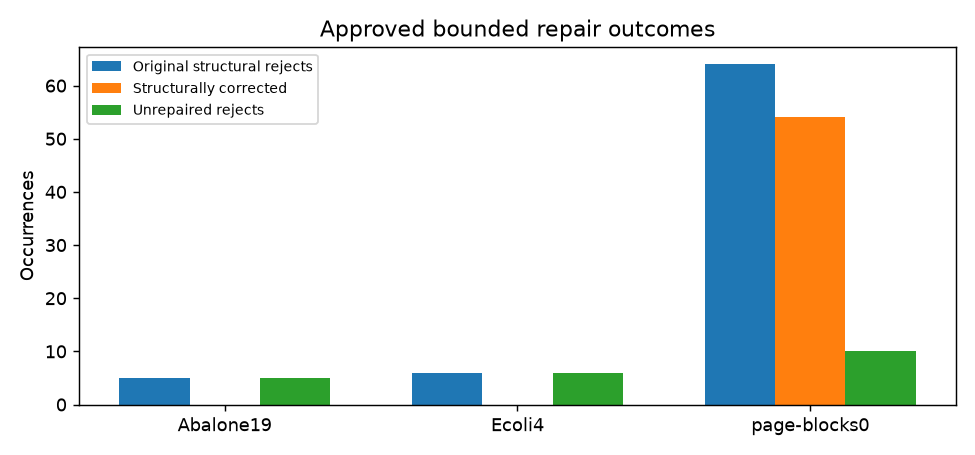
\includegraphics[width=.85\linewidth]{figures/repair-outcomes.png}\caption{Repair outcomes by original occurrence; structural correction is not human validity.}\label{fig:repair}\end{figure}
The largest observed absolute percentile shift is .0275 locally: page-blocks0 source occurrence 131 rounds height 4.5 to 4 and Lenght 32.5 to 32. Global percentile changes .0075; its action becomes provisional pass. This pool supplies no extreme evidence discontinuity. The report lists largest observed shifts without manufacturing a dramatic example.

\small\begin{longtable}{lrrrrr}
\caption{Matched middle-budget construction. C: distinct-feature TRAIN coverage; D: exact duplicate rate; N: near-duplicate rate. O: original pool; R: repair-augmented pool.}\label{tab:coverage}\\
\toprule
Dataset / strategy / pool & n & Derived & C & D & N \\
\midrule
\endfirsthead
\toprule
Dataset / strategy / pool & n & Derived & C & D & N \\
\midrule
\endhead
page-blocks0 / source-order / O & 49 & 0 & 0.9139 & 0.2653 & 0.5918 \\
page-blocks0 / source-order / R & 49 & 11 & 0.9099 & 0.1837 & 0.5918 \\
page-blocks0 / farthest-first / O & 49 & 0 & 0.9324 & 0.0000 & 0.0000 \\
page-blocks0 / farthest-first / R & 49 & 11 & 0.9359 & 0.0000 & 0.0000 \\
page-blocks0 / coverage-greedy / O & 49 & 0 & 0.9324 & 0.1633 & 0.4490 \\
page-blocks0 / coverage-greedy / R & 49 & 9 & 0.9370 & 0.0816 & 0.4082 \\
page-blocks0 / quality-coverage / O & 49 & 0 & 0.9324 & 0.0000 & 0.3265 \\
page-blocks0 / quality-coverage / R & 49 & 16 & 0.9370 & 0.0000 & 0.1020 \\
Ecoli4 / source-order / O & 70 & 0 & 0.4164 & 0.2000 & 0.3857 \\
Ecoli4 / source-order / R & 70 & 0 & 0.4164 & 0.2000 & 0.3857 \\
Ecoli4 / farthest-first / O & 70 & 0 & 0.4684 & 0.0000 & 0.0000 \\
Ecoli4 / farthest-first / R & 70 & 0 & 0.4684 & 0.0000 & 0.0000 \\
Ecoli4 / coverage-greedy / O & 70 & 0 & 0.5056 & 0.1143 & 0.2429 \\
Ecoli4 / coverage-greedy / R & 70 & 0 & 0.5056 & 0.1143 & 0.2429 \\
Ecoli4 / quality-coverage / O & 70 & 0 & 0.5056 & 0.0000 & 0.0000 \\
Ecoli4 / quality-coverage / R & 70 & 0 & 0.5056 & 0.0000 & 0.0000 \\
Abalone19 / source-order / O & 56 & 0 & 0.6225 & 0.3571 & 0.6250 \\
Abalone19 / source-order / R & 56 & 0 & 0.6225 & 0.3571 & 0.6250 \\
Abalone19 / farthest-first / O & 56 & 0 & 0.9401 & 0.0000 & 0.0000 \\
Abalone19 / farthest-first / R & 56 & 0 & 0.9401 & 0.0000 & 0.0000 \\
Abalone19 / coverage-greedy / O & 56 & 0 & 0.9479 & 0.1071 & 0.2679 \\
Abalone19 / coverage-greedy / R & 56 & 0 & 0.9479 & 0.1071 & 0.2679 \\
Abalone19 / quality-coverage / O & 56 & 0 & 0.9479 & 0.0000 & 0.0000 \\
Abalone19 / quality-coverage / R & 56 & 0 & 0.9479 & 0.0000 & 0.0000 \\
\bottomrule
\end{longtable}
\normalsize
Figure~\ref{fig:coverage} compares geometric coverage. The pool grows 451 to 500 through page-blocks0 (119 to 168). Original conditions exactly reproduce Phase 5. At page budget 49, quality-coverage selects 16 derived records: distinct-feature TRAIN coverage rises .9324 to .9370, near duplication falls .3265 to .1020, exact duplication remains zero. Source-order coverage slightly declines. Pool expansion does not guarantee a better fixed-budget set. The other datasets stay unchanged.

\begin{figure}[ht]\centering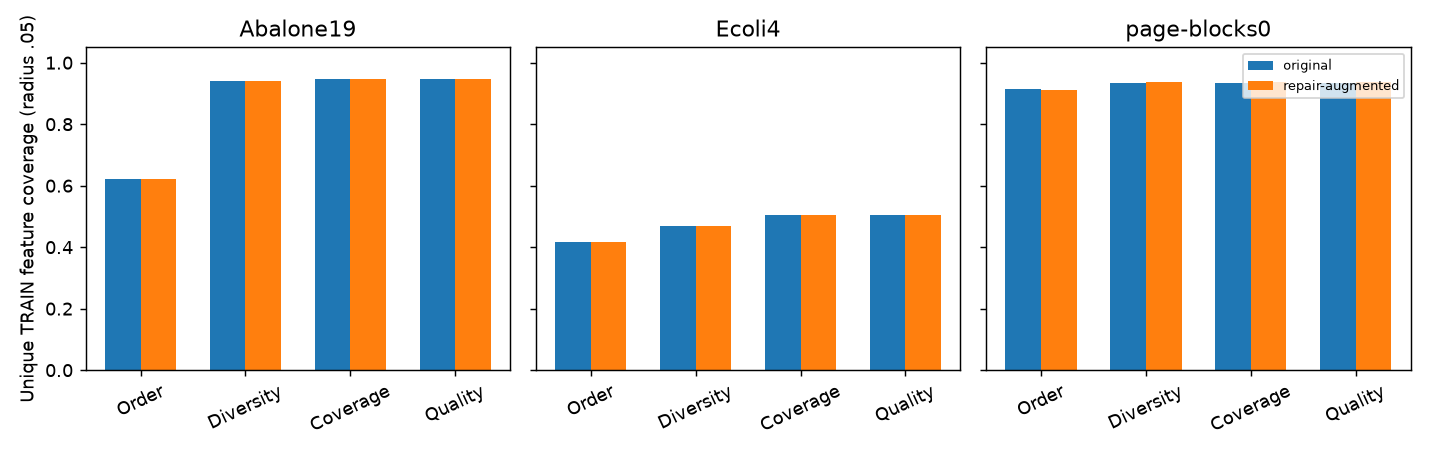
\includegraphics[width=\linewidth]{figures/coverage-comparison.png}\caption{Matched budgets; coverage describes TRAIN geometry, not accuracy.}\label{fig:coverage}\end{figure}

\subsection{Task utility and unavailable comparisons}
\small\begin{longtable}{lrrrr}
\caption{Fixed TEST task utility. L/F: logistic/random forest. QO/QR: quality-coverage original/repair pool. H: hybrid minority augmentation.}\label{tab:utility}\\
\toprule
Dataset / source / regime / model & F1 & AP & BA & MCC \\
\midrule
\endfirsthead
\toprule
Dataset / source / regime / model & F1 & AP & BA & MCC \\
\midrule
\endhead
Abalone19 / Real / TRTR / L & 0.0000 & 0.0256 & 0.5000 & 0.0000 \\
Abalone19 / Real / TRTR / F & 0.0000 & 0.0231 & 0.5000 & 0.0000 \\
Abalone19 / QO / TSTR / L & 0.0312 & 0.0191 & 0.7748 & 0.0933 \\
Abalone19 / QO / H / L & 0.0000 & 0.0170 & 0.5000 & 0.0000 \\
Abalone19 / QO / TSTR / F & 0.0303 & 0.0211 & 0.7240 & 0.0777 \\
Abalone19 / QO / H / F & 0.0000 & 0.0365 & 0.4994 & -0.0029 \\
Abalone19 / QR / TSTR / L & 0.0312 & 0.0191 & 0.7748 & 0.0933 \\
Abalone19 / QR / H / L & 0.0000 & 0.0170 & 0.5000 & 0.0000 \\
Abalone19 / QR / TSTR / F & 0.0303 & 0.0211 & 0.7240 & 0.0777 \\
Abalone19 / QR / H / F & 0.0000 & 0.0365 & 0.4994 & -0.0029 \\
Ecoli4 / Real / TRTR / L & 1.0000 & 1.0000 & 1.0000 & 1.0000 \\
Ecoli4 / Real / TRTR / F & 0.6667 & 1.0000 & 0.7500 & 0.6961 \\
Ecoli4 / QO / TSTR / L & 0.2051 & 0.1355 & 0.7540 & 0.2409 \\
Ecoli4 / QO / H / L & 1.0000 & 1.0000 & 1.0000 & 1.0000 \\
Ecoli4 / QO / TSTR / F & 0.2963 & 0.6326 & 0.8492 & 0.3485 \\
Ecoli4 / QO / H / F & 1.0000 & 1.0000 & 1.0000 & 1.0000 \\
Ecoli4 / QR / TSTR / L & 0.2051 & 0.1355 & 0.7540 & 0.2409 \\
Ecoli4 / QR / H / L & 1.0000 & 1.0000 & 1.0000 & 1.0000 \\
Ecoli4 / QR / TSTR / F & 0.2963 & 0.6326 & 0.8492 & 0.3485 \\
Ecoli4 / QR / H / F & 1.0000 & 1.0000 & 1.0000 & 1.0000 \\
page-blocks0 / Real / TRTR / L & 0.7150 & 0.7456 & 0.8019 & 0.6991 \\
page-blocks0 / Real / TRTR / F & 0.8692 & 0.9213 & 0.9106 & 0.8562 \\
page-blocks0 / QO / TSTR / L & 0.4464 & 0.5552 & 0.7590 & 0.3892 \\
page-blocks0 / QO / H / L & 0.7150 & 0.7444 & 0.8019 & 0.6991 \\
page-blocks0 / QO / TSTR / F & 0.3421 & 0.4468 & 0.7269 & 0.2880 \\
page-blocks0 / QO / H / F & 0.8626 & 0.9094 & 0.9022 & 0.8499 \\
page-blocks0 / QR / TSTR / L & 0.3421 & 0.5716 & 0.7129 & 0.2780 \\
page-blocks0 / QR / H / L & 0.7150 & 0.7423 & 0.8019 & 0.6991 \\
page-blocks0 / QR / TSTR / F & 0.3158 & 0.4742 & 0.7041 & 0.2544 \\
page-blocks0 / QR / H / F & 0.8732 & 0.9093 & 0.9111 & 0.8610 \\
\bottomrule
\end{longtable}
\normalsize
Of 138 rows, 114 return results and 24 are unavailable. The six source-order populations, each with two models/two regimes, contain no positive-literal synthetic records. No favorable substitute replaces an unavailable result. Full controls and other strategies remain in CSV/JSON.

Figure~\ref{fig:utility} shows the fixed logistic comparisons. Abalone19 TRTR F1 is zero for both models despite nonzero ranking metrics. Ecoli4 logistic TRTR reaches 1.0 on only four TEST positives, not proof of universal performance. Page quality-coverage logistic TSTR F1 falls .4464 to .3421 after repair-pool expansion while AP rises .5552 to .5716. Hybrid F1 remains .7150 and AP slightly falls. These mixed outcomes do not establish uniform improvement. No significance/interval is inferred from one split.

\begin{figure}[ht]\centering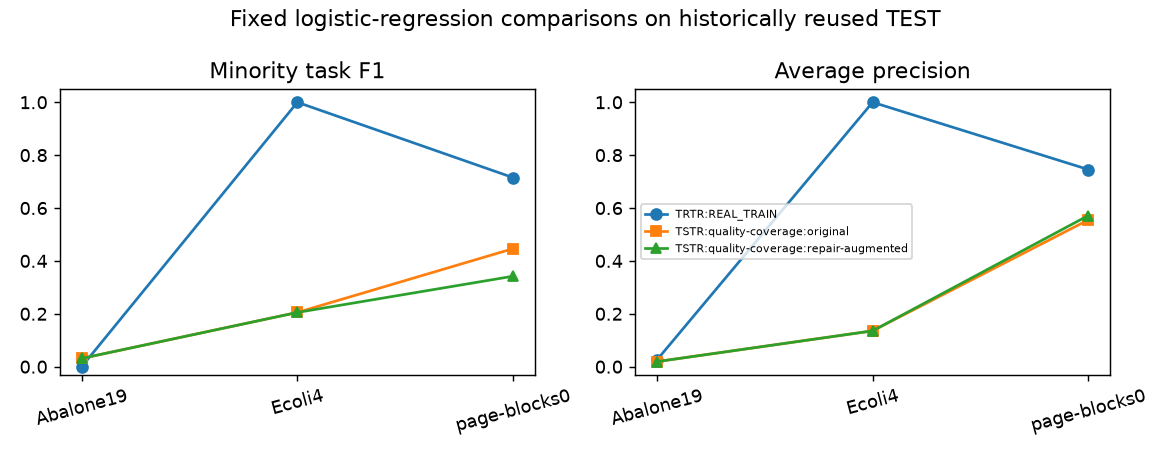
\includegraphics[width=\linewidth]{figures/task-utility.png}\caption{Fixed logistic comparisons on reused historical TEST. Connected points identify datasets, not an ordered trend.}\label{fig:utility}\end{figure}

\subsection{Reproducibility and runtime}
Repair records, constructions and task payloads replay exactly in new locations. Runtime envelopes need not share fingerprints; substantive content does. M2 replay covers 601 occurrences/three families. The registry contains 258 entries across controls, configurations, policies, original constructions, repair, new constructions and utility. Original 51-dataset audit evidence is retained rather than rerun.

Repair scoring takes about 2.590 seconds on this workstation, excluding context loading/construction. Utility runtime and dependencies are recorded; no hardware-general speed claim is made. Replay supplies no confidence interval. Final tests, static checks and historical hashes are recorded separately in closeout evidence.

\section{Discussion and limitations}
This study supports a narrow engineering conclusion: authoritative declarations, statistical support, set geometry, bounded editing and utility can be explicit and reproducible without conflating meanings. Repair addresses some observed defects while refusing missing labels and richer semantic problems. Eligibility is no evidence that broader repair would be safe.

The study is small and historical. Provider/critic outputs are recorded artifacts, not a new randomized generation campaign. Exact-value overlap and prior TEST evaluation limit independence claims. Two datasets have few positive TEST examples. Single-seed utility describes fixed comparisons only. Geometric gains do not establish causal utility benefits; unfavorable results remain evidence.

Authority is limited to justified declarations. Physical quantities, target mappings and cross-field rules remain unresolved where sources cannot substantiate them. Distances depend on scaling, sparse references and nonlinear/multimodal structure. Candidate percentiles are descriptive ranks, not probabilities. Max fusion avoids pretending independence but has no calibrated risk guarantee.

All 120 labels remain proposals: zero VALID, 27 INVALID, 93 INDETERMINATE. There are no human-final approvals. Official validity precision/recall, false acceptance/rejection, agreement and real calibration are unavailable. INDETERMINATE is not made positive/negative. This study cannot establish a genuinely valid synthetic population. Ledger fingerprints aid consistency, not authentication against malicious same-permission actors.

\section{Conclusion}
RC-QASyn implements six phases with frozen controls, source-bound evidence, descriptive policies, deterministic construction and bounded repair. Approved repair corrects 54 of 75 structural rejects and refuses 21; 49 derived versions meet unchanged provisional conditions. Coverage and task effects vary by method and metric. The record is inspectable and reproducible; scientific approval remains human responsibility.

\section{Future work and pending evidence}
Personal review of every cohort record and explicit reviewed-ledger confirmation come next. Only then can official B2/B3-versus-human analysis proceed; adequate independent class support must precede calibration. Authoritative semantics may refine future specifications but cannot be invented to reinterpret current outcomes. New datasets, generation, richer repair and learned fusion are outside this implementation. Future evaluation should predeclare comparisons, address value-level overlap and distinguish new evidence from reused TEST.

\section{Declarations and contribution placeholders}
\textbf{Authors/affiliations:} [HUMAN INPUT REQUIRED: names, institution, contact and order].

\textbf{Contributions:} [HUMAN INPUT REQUIRED: accurate CRediT roles for methodology, implementation, supervision and writing].

\textbf{Funding/conflicts:} [HUMAN INPUT REQUIRED; no absence is asserted].

\textbf{Data/code:} Local versioned source, provenance and experiments accompany this draft. Public release, licensing and venue wording require author review. No remote release is implied.

\textbf{Human review/ethics:} Validity review is pending. No completed institutional approval, exemption or independent annotation agreement is claimed. Human authors must determine requirements.

\textbf{AI assistance:} An AI coding/drafting assistant supported implementation, orchestration, source checking and manuscript preparation under researcher instructions. Human authors must review all results/references/claims, accept submission responsibility and confirm institutional/venue wording. No AI is an author.

\textbf{Scientific status:} Engineering completion differs from scientific acceptance. Claims, semantics, reviewed truth and official calibration remain pending. This is a research draft, not an approved publication or scientific freeze.

\bibliographystyle{plainnat}
\bibliography{references}
\appendix
\section{Complete primary construction budgets}
\small\begin{longtable}{lrrrr}
\caption{Original Phase-5 primary budget matrix. C: distinct-feature TRAIN coverage.}\label{tab:phase5}\\
\toprule
Dataset / strategy & Budget & C & Exact & Near \\
\midrule
\endfirsthead
\toprule
Dataset / strategy & Budget & C & Exact & Near \\
\midrule
\endhead
Abalone19 / source-order & 28 & 0.5883 & 0.2857 & 0.5357 \\
Abalone19 / farthest-first & 28 & 0.8572 & 0.0000 & 0.0000 \\
Abalone19 / coverage-greedy & 28 & 0.9383 & 0.0000 & 0.0000 \\
Abalone19 / quality-coverage & 28 & 0.9368 & 0.0000 & 0.0000 \\
Abalone19 / source-order & 56 & 0.6225 & 0.3571 & 0.6250 \\
Abalone19 / farthest-first & 56 & 0.9401 & 0.0000 & 0.0000 \\
Abalone19 / coverage-greedy & 56 & 0.9479 & 0.1071 & 0.2679 \\
Abalone19 / quality-coverage & 56 & 0.9479 & 0.0000 & 0.0000 \\
Abalone19 / source-order & 84 & 0.6746 & 0.3929 & 0.7262 \\
Abalone19 / farthest-first & 84 & 0.9467 & 0.0000 & 0.0000 \\
Abalone19 / coverage-greedy & 84 & 0.9479 & 0.1905 & 0.3810 \\
Abalone19 / quality-coverage & 84 & 0.9479 & 0.0000 & 0.0000 \\
Ecoli4 / source-order & 35 & 0.3717 & 0.1714 & 0.2857 \\
Ecoli4 / farthest-first & 35 & 0.4164 & 0.0000 & 0.0000 \\
Ecoli4 / coverage-greedy & 35 & 0.5056 & 0.0571 & 0.1143 \\
Ecoli4 / quality-coverage & 35 & 0.5056 & 0.0000 & 0.0000 \\
Ecoli4 / source-order & 70 & 0.4164 & 0.2000 & 0.3857 \\
Ecoli4 / farthest-first & 70 & 0.4684 & 0.0000 & 0.0000 \\
Ecoli4 / coverage-greedy & 70 & 0.5056 & 0.1143 & 0.2429 \\
Ecoli4 / quality-coverage & 70 & 0.5056 & 0.0000 & 0.0000 \\
Ecoli4 / source-order & 105 & 0.4610 & 0.2000 & 0.3714 \\
Ecoli4 / farthest-first & 105 & 0.5019 & 0.0000 & 0.0000 \\
Ecoli4 / coverage-greedy & 105 & 0.5056 & 0.2000 & 0.3524 \\
Ecoli4 / quality-coverage & 105 & 0.5056 & 0.0000 & 0.0000 \\
page-blocks0 / source-order & 24 & 0.8713 & 0.1250 & 0.3750 \\
page-blocks0 / farthest-first & 24 & 0.9315 & 0.0000 & 0.0000 \\
page-blocks0 / coverage-greedy & 24 & 0.9324 & 0.0000 & 0.0833 \\
page-blocks0 / quality-coverage & 24 & 0.9319 & 0.0000 & 0.0833 \\
page-blocks0 / source-order & 49 & 0.9139 & 0.2653 & 0.5918 \\
page-blocks0 / farthest-first & 49 & 0.9324 & 0.0000 & 0.0000 \\
page-blocks0 / coverage-greedy & 49 & 0.9324 & 0.1633 & 0.4490 \\
page-blocks0 / quality-coverage & 49 & 0.9324 & 0.0000 & 0.3265 \\
page-blocks0 / source-order & 74 & 0.9264 & 0.2027 & 0.6622 \\
page-blocks0 / farthest-first & 74 & 0.9324 & 0.0000 & 0.5946 \\
page-blocks0 / coverage-greedy & 74 & 0.9324 & 0.2027 & 0.6081 \\
page-blocks0 / quality-coverage & 74 & 0.9324 & 0.0000 & 0.5676 \\
\bottomrule
\end{longtable}
\normalsize
\section{Reproduction and evidence map}
The repository document \texttt{docs/phase6-m6-m9-methods.md} gives exact commands. The core CLI restores saved evidence parameters, writes immutable derived records and constructs matched-budget datasets. The utility CLI runs only predeclared task comparisons. Reporting reads sealed results without fitting. The final reproducibility manifest binds dependencies, source files, split identities, configuration versions, commands and artifact hashes. Canonical object fingerprints and raw-file SHA-256 hashes are distinguished.

The table ledger \texttt{notes/table-evidence.json} records every cell, source field and row fingerprint. Full edits, raw/normalized scores and source ordinals remain in the repair bundle. Full task results, including unavailable cases, are distributed as CSV/JSON. Author and supervisor review is required before submission or scientific freeze.
\end{document}
